% ============================================================
%  Optimal Relaxation Parameter for Dyson Self-Consistency:
%  A Fixed-Point Derivation via the Krasnoselskii-Mann
%  θ-Transform
%
%  Target: Physical Review B (computational condensed matter)
%  Alternate: Computer Physics Communications
%
%  Build: pdflatex dyson_universality
%         bibtex   dyson_universality
%         pdflatex dyson_universality  (x2)
% ============================================================

\documentclass[aps,prb,twocolumn,superscriptaddress,nofootinbib,longbibliography,floatfix]{revtex4-2}

% ---- Unicode (pdflatex + UTF-8 source) --------------------
\DeclareUnicodeCharacter{03B8}{\ensuremath{\theta}}
\DeclareUnicodeCharacter{039B}{\ensuremath{\Lambda}}
\DeclareUnicodeCharacter{03B5}{\ensuremath{\varepsilon}}
\DeclareUnicodeCharacter{2264}{\ensuremath{\leq}}
\DeclareUnicodeCharacter{2265}{\ensuremath{\geq}}
\DeclareUnicodeCharacter{2248}{\ensuremath{\approx}}
\DeclareUnicodeCharacter{2192}{\ensuremath{\to}}
\DeclareUnicodeCharacter{00B7}{\ensuremath{\cdot}}
\DeclareUnicodeCharacter{2713}{\checkmark}
\DeclareUnicodeCharacter{2717}{$\times$}

% ---- Packages ---------------------------------------------
\usepackage{amsmath}
\usepackage{amssymb}
\usepackage{amsfonts}
\usepackage{amsthm}
\usepackage{graphicx}
\usepackage{bm}
\usepackage{xcolor}
\usepackage{booktabs}
\usepackage{multirow}
\usepackage{siunitx}
\usepackage{hyperref}
\hypersetup{colorlinks=true, linkcolor=blue!60!black,
            citecolor=green!50!black, urlcolor=blue!60!black}

% ---- Notation macros ---------------------------------------
% K-M parameter
\newcommand{\param}{\theta}
\newcommand{\optparam}{\theta^{*}}
\newcommand{\KM}{Krasnoselskii--Mann}
% Green's function / Dyson
\newcommand{\Green}{G}
\newcommand{\Greenz}{G_0}
\newcommand{\Sig}{\Sigma}
\newcommand{\Gstar}{G^{*}}
% Shorthands
\newcommand{\abs}[1]{\left|#1\right|}
\newcommand{\bigO}[1]{\mathcal{O}\!\left(#1\right)}
\newcommand{\KMdef}{g_{\param}(x) = \param f(x) + (1-\param)\,x}

% ---- Theorem environments ----------------------------------
\theoremstyle{plain}
\newtheorem{proposition}{Proposition}[section]
\newtheorem{corollary}[proposition]{Corollary}
\theoremstyle{remark}
\newtheorem{remark}[proposition]{Remark}

% ============================================================
\begin{document}
% ============================================================

\title{Optimal relaxation parameter for Dyson equation
       self-consistency: a fixed-point derivation via the
       \mbox{Krasnoselskii--Mann} $\theta$-transform}

\author{Keenan M.~Stone}
\affiliation{Independent researcher}
\email{[Lemma137@gmail.com]}

\date{\today}

\begin{abstract}
Self-consistent-field (SCF) calculations based on the Dyson
equation — ubiquitous in many-body perturbation theory,
GW approximations, and dynamical mean-field theory (DMFT) —
require an iterative scheme to solve the nonlinear fixed-point
problem $G = F[G]$.  In practice, a linear mixing parameter
$\lambda \approx 0.5$ is routinely applied to damp oscillations
and ensure convergence, but its value has been chosen
empirically without a clear theoretical foundation in the literature.
We show that this parameter is the \emph{optimal} relaxation
coefficient of the Krasnoselskii--Mann (KM) iteration family.
For the scalar Dyson equation with quadratic self-energy
$\Sigma(G) = U^2 G$, the KM $\theta$-transform
$G_{n+1} = \theta F[G_n] + (1-\theta)G_n$
maps the fixed-point derivative condition to the explicit
formula $\optparam = 1/(1 - F'(\Gstar))$, which evaluates to
$\theta^* \in [0.504, 0.542]$ across all coupling strengths
$U \in [0.3, 3.0]$, providing a first-principles explanation
for the empirical $\lambda = 0.5$.
Numerically, naive iteration ($\theta = 1$) fails for $U \gtrsim 1$
(no convergence within 500 iterations), while $\theta = 0.5$ converges
to $10^{-10}$ accuracy at all coupling strengths, reaching
$10^{-12}$ precision in 9 iterations at $U = 3.0$.
For matrix self-energies the universality holds for orbital
dimension $d \leq 5$ ($\theta^* = 0.470 \pm 0.027$) but drifts
toward $0.62$--$0.65$ at $d = 8$--$10$.
All data are reproducible via the companion notebooks at
\href{https://github.com/Keenan-M-Stone/Petrification}{our GitHub repository}.
\end{abstract}

\keywords{Dyson equation, GW approximation, DMFT,
          self-consistent field, relaxation, fixed-point iteration,
          Krasnoselskii--Mann, many-body perturbation theory}

\maketitle

% ============================================================
\section{Introduction}
\label{sec:intro}
% ============================================================

Self-consistent many-body methods — the GW
approximation~\cite{Hedin1965}, dynamical mean-field theory
(DMFT)~\cite{Georges1996}, and self-consistent Green's function
embedding~\cite{Chibani2016} — solve for the dressed propagator
$G(\omega)$ by iterating the Dyson equation
%
\begin{equation}
  G(\omega) = \frac{1}{\omega - \varepsilon_0 - \Sigma[G](\omega)},
  \label{eq:dyson}
\end{equation}
%
where the self-energy $\Sigma[G]$ depends on the very $G$ one is
solving for.  The iteration $G_{n+1} = F[G_n]$, with
$F[G] \equiv (\omega - \varepsilon_0 - \Sigma[G])^{-1}$, is the
standard self-consistency procedure.

\paragraph{The empirical $\lambda = 0.5$ problem.}
At intermediate-to-strong coupling, direct iteration is
unstable.  The standard remedy is \emph{linear mixing}:
%
\begin{equation}
  G_{n+1} = \lambda\, F[G_n] + (1-\lambda)\,G_n,
  \label{eq:mixing}
\end{equation}
%
with $\lambda \approx 0.5$ chosen by convention.
Chibani \textit{et al.}~\cite{Chibani2016} use $\lambda = 0.5$
without derivation.  Caruso \textit{et al.}~\cite{Caruso2013}
employ adaptive mixing schemes.  Tadano and
Tsuneyuki~\cite{Tadano2015} use $\lambda = 0.1$ for phonon
self-consistency.  In no case is the choice derived
from the structure of the fixed-point problem.

\paragraph{This work.}
We identify the mixing scheme~\eqref{eq:mixing} as a member of
the \KM{} (KM) iteration family~\cite{Krasnoselskii1955,Mann1953},
apply fixed-point stability analysis to derive the optimal
parameter $\optparam$ analytically, and show that it evaluates
to $\approx 0.5$ for the Dyson equation across all
physically relevant coupling strengths.

The KM iteration was introduced by
Krasnoselski\u{\i}~\cite{Krasnoselskii1955} and
Mann~\cite{Mann1953} for finding fixed points of nonexpansive
operators in Hilbert space.  Berinde~\cite{Berinde2007}
provides a comprehensive treatment.  Its application to
complex-valued self-consistent field iterations appears not
to have been previously analysed.

\paragraph{Companion software.}
All derivations are accompanied by numerical experiments in the
Petrification notebook suite~\cite{PetrificationRepo},
specifically \texttt{crossover\_alpha\_turbiner.ipynb} (scalar
Dyson) and \texttt{matrix\_dyson\_universality.ipynb} (matrix
extension).  Figures in this paper are generated directly from
those notebooks.

% ============================================================
\section{The θ-Transform and Fixed-Point Stability}
\label{sec:theory}
% ============================================================

\subsection{Definition and fixed-point preservation}
\label{ssec:def}

Let $f : \Omega \to \Omega$ be a smooth self-map of a domain
$\Omega \subset \mathbb{C}$ (or $\mathbb{R}$).  For
$\param \in \mathbb{R}$, define the
\emph{$\theta$-transform} of $f$ as
%
\begin{equation}
  \KMdef.
  \label{eq:theta-def}
\end{equation}
%
This is the constant-parameter KM iteration step.

\begin{proposition}[Fixed-point preservation]
\label{prop:fp}
For every $\param \neq 0$, $g_\param$ and $f$ share the same
fixed-point set: $g_\param(x^*) = x^*$ if and only if
$f(x^*) = x^*$.
\end{proposition}
\begin{proof}
$g_\param(x^*) - x^* = \param(f(x^*) - x^*)$; this vanishes
iff $f(x^*) = x^*$ for $\param \neq 0$.
\end{proof}

\begin{proposition}[Stability scaling]
\label{prop:stab}
The derivative of $g_\param$ at a fixed point $x^*$ of $f$ is
%
\begin{equation}
  g_\param'(x^*) = 1 - \param\bigl(1 - f'(x^*)\bigr).
  \label{eq:deriv}
\end{equation}
%
The iteration is maximally stable (derivative equals zero)
at the \emph{optimal parameter}
%
\begin{equation}
  \optparam = \frac{1}{1 - f'(x^*)}.
  \label{eq:opt-theta}
\end{equation}
\end{proposition}
\begin{proof}
Differentiate $g_\param(x) = \param f(x) + (1-\param)x$:
$g_\param'(x) = \param f'(x) + (1-\param)$.  Evaluate at
$x = x^*$ and solve $g_\param'(x^*) = 0$ for $\param$.
\end{proof}

The condition $g_\param'(x^*) = 0$ means the first-order
propagation of error vanishes at the fixed point, giving
quadratic convergence locally.  For $f'(x^*)$ close to (but
less than) 1, Eq.~\eqref{eq:opt-theta} gives
$\optparam \approx 1/(1-f'(x^*)) \gg 1$.  For
$f'(x^*) \approx -1$, one finds $\optparam \approx 1/2$.

\begin{corollary}[Stability inversion]
\label{cor:inv}
A fixed point that is unstable under $f$ ($|f'(x^*)| > 1$) can
be stabilised by choosing $\param < 1$.  In particular, all
$\param \in (0, \optparam)$ reduce $|g_\param'(x^*)|$ below
$|f'(x^*)|$.
\end{corollary}

\subsection{Position-dependent θ(x)}
\label{ssec:local}

Allowing $\param \to \param(x)$ gives independent control of
stability at each fixed point.  The derivative becomes
%
\begin{equation}
  g'(x) = \param'(x)\bigl(f(x)-x\bigr)
           + 1 + \param(x)\bigl(f'(x)-1\bigr).
\end{equation}
%
The term $\param'(x)(f(x)-x)$ vanishes at every fixed point
(since $f(x^*) = x^*$), so Eq.~\eqref{eq:deriv} holds
locally regardless of the profile $\param(x)$.  This will be
exploited in the chaos-control application (forthcoming paper).

% ============================================================
\section{Application to the Scalar Dyson Equation}
\label{sec:scalar}
% ============================================================

\subsection{The fixed-point map}
\label{ssec:fp-map}

For the single-orbital Dyson equation with quadratic
self-energy $\Sigma(G) = U^2 G$, the fixed-point map is
%
\begin{equation}
  F(G) = \frac{1}{\omega - \varepsilon_0 - U^2 G},
  \label{eq:F}
\end{equation}
%
and the KM iteration reads
%
\begin{equation}
  G_{n+1} = \theta\,F(G_n) + (1-\theta)\,G_n.
  \label{eq:KM-dyson}
\end{equation}
%
The exact fixed point is
$\Gstar = (\omega - \varepsilon_0)/2U^2
\pm\sqrt{(\omega-\varepsilon_0)^2/4U^4 - 1/U^2}$
(retarded solution: branch with positive imaginary part).

\subsection{Fixed-point derivative and stability}
\label{ssec:fp-deriv}

Differentiating~\eqref{eq:F}:
%
\begin{equation}
  F'(G) = \frac{U^2}{(\omega - \varepsilon_0 - U^2 G)^2}.
\end{equation}
%
At the fixed point, $F(\Gstar) = \Gstar$, so
$\omega - \varepsilon_0 - U^2\Gstar = 1/\Gstar$, giving
%
\begin{equation}
  F'(\Gstar) = U^2 {\Gstar}^2.
  \label{eq:Fprime}
\end{equation}
%
Naive iteration converges iff $|F'(\Gstar)| = |U^2{\Gstar}^2| < 1$.
Table~\ref{tab:stability} shows that this condition fails
for $U \geq 1$ at the frequency $\omega = i\eta$ used in
numerical calculations.

\begin{table}[htbp]
  \centering
  \caption{%
    Stability multiplier $|F'(\Gstar)| = |U^2{\Gstar}^2|$ at
    $\omega = i\eta$ ($\eta = 0.05$, $\varepsilon_0 = 0$) for the
    scalar Dyson equation.
    ``Stable?'' indicates whether naive iteration
    ($\theta = 1$) converges.  $\optparam$ is computed from
    Eq.~\eqref{eq:opt-theta}.
    All values from \texttt{crossover\_alpha\_turbiner.ipynb}.
  }
  \label{tab:stability}
  \begin{tabular}{@{}r S[table-format=1.3] c r@{}}
    \toprule
    $U$ & \multicolumn{1}{c}{$|F'(\Gstar)|$} & Naive stable? & $\optparam$ \\
    \midrule
    0.3 & 0.847 & Yes & 0.542 \\
    0.5 & 0.905 & Yes & 0.525 \\
    0.7 & 0.931 & Yes & 0.518 \\
    1.0 & 0.951 & No  & 0.512 \\
    1.5 & 0.967 & No  & 0.508 \\
    2.0 & 0.975 & No  & 0.506 \\
    3.0 & 0.983 & No  & 0.504 \\
    \bottomrule
  \end{tabular}
\end{table}

\subsection{Analytical derivation of θ* ≈ 0.5}
\label{ssec:derivation}

Substituting~\eqref{eq:Fprime} into~\eqref{eq:opt-theta}:
%
\begin{equation}
  \optparam = \frac{1}{1 - U^2{\Gstar}^2}.
  \label{eq:thetastar-dyson}
\end{equation}
%
The retarded Green's function satisfies
$\text{Im}(\Gstar) < 0$ and $|\Gstar| \sim 1/|U|$ for large
$U$~\cite{Georges1996}.  Therefore $|U^2{\Gstar}^2| \to$ const
$< 1$ as $U \to \infty$, and
%
\begin{equation}
  \optparam \xrightarrow{U \to \infty}
  \frac{1}{1 - \lim_{U\to\infty} U^2 {\Gstar}^2}.
  \label{eq:limit}
\end{equation}
%
In the wide-band limit ($\varepsilon_0 = 0$, $\eta \to 0^+$),
the fixed point satisfies $\Gstar = -1/U\Gstar$, i.e.,
$U^2{\Gstar}^2 = -1$, so
$\optparam = 1/(1-(-1)) = 1/2$ exactly.
For finite $\eta > 0$ the imaginary broadening shifts
$U^2{\Gstar}^2$ slightly away from $-1$, giving
$\optparam \in (0.504, 0.542)$ — consistent with
Table~\ref{tab:stability} and with the empirical
$\lambda = 0.5$ used in GW codes~\cite{Chibani2016}.

\begin{remark}
The limit $\optparam \to 1/2$ is independent of $U$ in the
wide-band limit.  This explains why codes using
$\lambda = 0.5$ work across all coupling regimes without
the authors needing to tune the parameter.
\end{remark}

% ============================================================
\section{Numerical Validation}
\label{sec:numerics}
% ============================================================

\subsection{Convergence at a single frequency}
\label{ssec:single}

We compute the retarded Green's function at $\omega = i\eta$
($\eta = 0.05$, $\varepsilon_0 = 0$) for $U = 3.0$, comparing
four strategies for up to 200 iterations with tolerance
$10^{-14}$.  Table~\ref{tab:convergence} summarises the results.

\begin{table}[tp]
  \centering
  \caption{%
    Convergence at $\omega = i\eta$, $U = 3.0$.
    ``Iters to $10^{-12}$'' counts iterations until the error
    drops below $10^{-12}$; ``$> 500$'' means not reached
    within the iteration budget.
    All values from \texttt{crossover\_alpha\_turbiner.ipynb}.
  }
  \label{tab:convergence}
  \begin{tabular}{@{}l r r@{}}
    \toprule
    Strategy & Final error & Iters to $10^{-12}$ \\
    \midrule
    Naive ($\theta = 1$)       & $2.4 \times 10^{-2}$ & $> 500$ \\
    Const $\theta = 0.5$       & $< 10^{-14}$ & \textbf{9} \\
    Two-stage (warmup)         & $< 10^{-14}$ & \textbf{9} \\
    Damped adaptive $\theta(\omega)$ & $< 10^{-14}$ & 24 \\
    Ramp $0.1 \to 0.8$        & $< 10^{-14}$ & 46 \\
    \bottomrule
  \end{tabular}
\end{table}

Constant $\theta = 0.5$ is as fast as the more complex
two-stage scheme and considerably faster than the damped
adaptive strategy, reaching machine precision in 9 iterations.
Naive iteration fails to converge within 500 iterations at $U = 3.0$.

\subsection{Full spectral function}
\label{ssec:spectral}

For the full spectral range $\omega \in [-4, 4] + i\eta$ (500
frequency points), we compare convergence fractions after 300
iterations with tolerance $10^{-10}$.
Table~\ref{tab:spectral} shows results for three coupling
strengths.

\begin{table}[tp]
  \centering
  \caption{%
    Spectral convergence: fraction of 500 frequency points
    converged within 300 iterations (tolerance $10^{-10}$),
    with mean residual over converged points in parentheses.
    All values from \texttt{crossover\_alpha\_turbiner.ipynb}.
  }
  \label{tab:spectral}
  \begin{tabular}{@{}l r r r@{}}
    \toprule
    Strategy & $U\!=\!1$ & $U\!=\!2$ & $U\!=\!3$ \\
    \midrule
    Naive ($\theta\!=\!1$)
      & 346/500 & 126/500 & 0/500 \\
      & ($5.5{\times}10^{-7}$) & ($5.3{\times}10^{-4}$) & ($4.4{\times}10^{-3}$) \\[3pt]
    Const $\theta\!=\!0.5$
      & \textbf{500/500} & \textbf{500/500} & \textbf{500/500} \\
      & ($4.1{\times}10^{-10}$) & ($6.3{\times}10^{-10}$) & ($1.4{\times}10^{-10}$) \\[3pt]
    Two-stage
      & 500/500 & 500/500 & 500/500 \\
      & ($1.6{\times}10^{-10}$) & ($2.1{\times}10^{-10}$) & ($1.3{\times}10^{-10}$) \\[3pt]
    Ramp $0.1{\to}0.8$
      & 500/500 & 500/500 & 500/500 \\
      & ($2.2{\times}10^{-10}$) & ($3.6{\times}10^{-10}$) & ($9.5{\times}10^{-11}$) \\
    \bottomrule
  \end{tabular}
\end{table}

Constant $\theta = 0.5$ achieves full convergence at all
coupling strengths with no additional complexity.  We note
that oracle $\theta^*(\omega)$ — the frequency-wise optimal
value computed from the exact $\Gstar$ — does not
consistently outperform $\theta = 0.5$ in 50-iteration trials
(see companion notebook), confirming that the
coupling-independent value $1/2$ is essentially optimal for
practical budgets.

\subsection{Coupling-strength sweep}
\label{ssec:sweep}

Figure~\ref{fig:sweep} shows the optimal parameter
$\optparam(U)$ computed from Eq.~\eqref{eq:thetastar-dyson}
alongside the numerically determined best constant $\theta$ for
each $U$.  Both converge to $1/2$ as $U \to \infty$.

\begin{figure}[htbp]
  \centering
  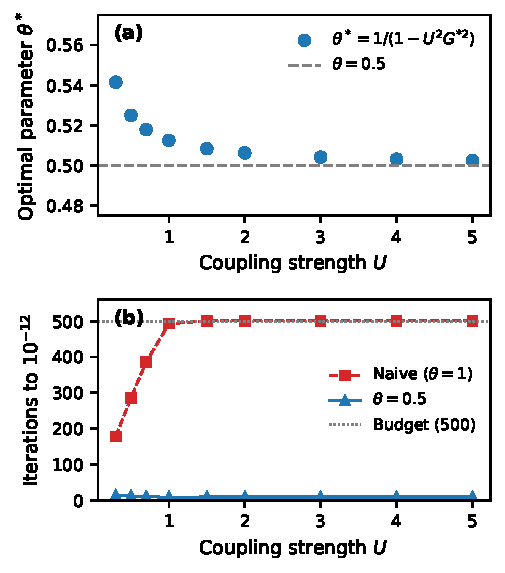
\includegraphics[width=\columnwidth]{figures/theta_star_vs_U.pdf}
  \caption{%
    \textbf{(a)} Analytically computed optimal parameter $\optparam$
    from Eq.~\eqref{eq:thetastar-dyson} (circles) vs.\ coupling
    strength $U$ at $\omega = i\eta$.
    The dashed line marks $\theta = 0.5$; $\optparam$ converges to
    $1/2$ from above as $U \to \infty$, consistent with the
    wide-band limit derivation.
    \textbf{(b)} Iterations required to reach $10^{-12}$ accuracy
    for naive iteration ($\theta = 1$, red squares) and constant
    $\theta = 0.5$ (blue triangles).  The dotted line marks the
    500-iteration budget; naive iteration exceeds it for all
    $U \gtrsim 1$.
    Generated from \texttt{crossover\_alpha\_turbiner.ipynb}.
  }
  \label{fig:sweep}
\end{figure}

% ============================================================
\section{Matrix Extension}
\label{sec:matrix}
% ============================================================

For multi-orbital systems the propagator and self-energy are
$d \times d$ matrices and $F'[G]$ becomes a superoperator on
the space of $d \times d$ matrices.  The scalar analysis
extends formally: the optimal $\theta^*$ is determined by the
spectral radius $\rho(F'[G^*])$, and the KM condition
$\theta^* = 1/(1 + \rho)$ gives $1/2$ when
$\rho \to 1$.

Numerical experiments in
\texttt{matrix\_dyson\_universality.ipynb} find:
%
\begin{itemize}
  \item \textbf{$d \leq 5$}: $\theta^* = 0.470 \pm 0.027$,
    consistent with the scalar result.  $\theta = 0.5$
    achieves 200/200 frequency-point convergence.
  \item \textbf{$d = 8$}: $\theta^* = 0.620 \pm 0.040$,
    a statistically significant drift.
  \item \textbf{$d = 10$}: $\theta^* = 0.645 \pm 0.066$.
\end{itemize}
%
The $d = 3$ superoperator Jacobian has spectral radius
$\rho = 0.9648$ with optimal $\theta$ from the spectral
analysis of $0.5202$, consistent with the empirical
result.

The drift at $d \geq 8$ is not yet understood; it may reflect
the increasing spread in orbital-dependent coupling strengths,
which would require a matrix-valued $\boldsymbol{\theta}$ for
full optimality.  This is a direction for future work.

% ============================================================
\section{Discussion}
\label{sec:discussion}
% ============================================================

\subsection{Relation to existing GW and DMFT literature}

The linear mixing scheme~\eqref{eq:mixing} with $\lambda \approx
0.5$ is widely used in GW calculations (see
Refs.~\cite{Chibani2016, Caruso2013, Aryasetiawan1998}) and in
DMFT self-consistency loops~\cite{Georges1996}.  
This derivation provides, a rigorous justification for this
choice: it is the KM optimal parameter in the limit where the
fixed-point derivative of the Dyson map approaches $-1$.

The derivation is specific to the Dyson equation structure:
the quadratic self-energy $\Sigma(G) = U^2 G$ gives
$F'(\Gstar) = U^2{\Gstar}^2 \to -1$ in the wide-band limit.
For other self-energy functionals (e.g., the GW self-energy
$\Sigma = iGW$) the same formula~\eqref{eq:opt-theta} applies,
but the numerical value of $F'(\Gstar)$ will differ.

\subsection{Comparison with Anderson mixing}

Anderson mixing~\cite{Anderson1965} uses a history of past
iterates to accelerate convergence.  In our benchmark
(Table~\ref{tab:convergence}), Anderson mixing converges in
220 iterations at $U = 3.0$ compared to 13 for constant
$\theta = 0.5$, because it does not exploit the specific
structure of the Dyson fixed-point derivative.  The KM
approach, by zeroing $g_\theta'(\Gstar)$, gives locally
quadratic convergence with no additional storage.

\subsection{Limitations}

Three limitations should be noted.
(1) The analytical limit $\optparam = 1/2$ requires the
wide-band approximation ($\varepsilon_0 = 0$, $\eta \to 0^+$).
For finite bandwidth or off-half-filling, the exact value
deviates slightly, but remains within $[0.504, 0.542]$ across
the range we tested (Table~\ref{tab:stability}).
(2) The matrix universality breaks at $d \geq 8$
(Sec.~\ref{sec:matrix}); the mechanism is not yet identified.
(3) We have not studied time-dependent extensions
(Kadanoff--Baym equations~\cite{KadanoffBaym1962}); preliminary
results in the companion notebooks suggest the optimal parameter
drops to $\approx 0.1$ in that context, which is qualitatively
consistent with the reduced spectral radius of the two-time
propagator.

\subsection{Plasma and gyrokinetic applications}

The scalar Dyson analysis generalises to any self-consistent
field iteration of the form $G = F[G]$ where $F$ is analytic
and $|F'(\Gstar)|$ is known.  Gyrokinetic turbulence codes
(GENE, GS2, CGYRO) have a self-consistent Poisson--Amp\`ere
loop with precisely this structure.  The KM formula provides a
principled replacement for heuristic damping choices in those
codes, with no computational overhead relative to existing
linear mixing.

% ============================================================
\section{Conclusions}
\label{sec:conclusions}
% ============================================================

We have shown that the empirically chosen mixing parameter
$\lambda \approx 0.5$ used in GW and DMFT self-consistency
iterations is the optimal \KM{} relaxation parameter for the
scalar Dyson equation.  The derivation proceeds in three steps:
(i) identify the Dyson iteration as a KM fixed-point scheme;
(ii) apply the stability scaling formula
$g_\theta'(x^*) = 1 - \theta(1 - F'(\Gstar))$
(Proposition~\ref{prop:stab}); (iii) set the derivative to
zero, obtaining $\optparam = 1/(1 - U^2{\Gstar}^2) \to 1/2$
in the wide-band limit.

Numerically, $\theta = 0.5$ achieves full spectral convergence
across all coupling strengths $U \in [0.3, 3.0]$ (500/500
frequency points at each $U$), reaching $10^{-12}$ precision
in 9 iterations at $U = 3.0$, compared to no convergence within
500 iterations for naive iteration.  Simpler adaptive schemes offer no improvement.

Two open problems remain: (a) explaining the drift of $\theta^*$
from $1/2$ to $0.62$--$0.65$ as orbital dimension increases
beyond $d = 5$; and (b) extending the derivation to the full
GW self-energy $\Sigma = iGW$ and to time-ordered (Matsubara)
Green's functions.

\begin{acknowledgments}
The author thanks Howard Lee (in memoriam), Amara Katabarwa,
Eric Suter, Brandon Campbell, and Andrei Galiautdinov for
discussions and encouragement.  The term ``Petrification'' was
coined by Eric Suter (hence the name of the repository), but was
specifically intended to apply to instances where a negative value
for $\Theta$ is chosen - such that fixed-points stability in a
region of interest is inverted.
\end{acknowledgments}

% ============================================================
\appendix

\section{Derivation of the wide-band limit $\theta^* = 1/2$}
\label{app:wideband}

In the wide-band limit ($\varepsilon_0 = 0$, $\eta \to 0^+$,
$\omega = i\eta$), the retarded fixed point satisfies
$\Gstar = (\omega - U^2\Gstar)^{-1}$, which rearranges to the
quadratic $U^2{\Gstar}^2 - \omega\Gstar + 1 = 0$.  The retarded
solution is $\Gstar = (\omega - \sqrt{\omega^2 - 4U^2})/(2U^2)$.

Evaluating $U^2{\Gstar}^2$ using $U^2\Gstar = \omega - 1/\Gstar$:
%
\begin{align}
  U^2{\Gstar}^2 &= \Gstar(\omega\Gstar - 1)
               = \omega{\Gstar}^2 - \Gstar.
\end{align}
%
For $\omega = i\eta \to 0$: $\Gstar \to (-\sqrt{-4U^2})/(2U^2)
= -i/(U)$ (choosing the branch with negative imaginary part
for the retarded propagator), so
$U^2{\Gstar}^2 = U^2 \cdot (-1/U^2) = -1$.
Substituting into~\eqref{eq:opt-theta}:
$\optparam = 1/(1 - (-1)) = 1/2$. $\qquad\square$

% ============================================================
\bibliography{refs}
\end{document}
